\chapter{Estado del arte}
\section{Introducción}
En este capítulo, se abordará el estado del arte en
cuanto a aplicaciones móviles para la colaboración y
actividades en grupo, destacando las características y
funcionalidades más relevantes de las soluciones existentes.
Además, se discutirán las áreas donde estas aplicaciones
presentan oportunidades de mejora y cómo nuestra propuesta
busca abordar dichas brechas.

\section{Estado del arte}
\subsection{Meetup}
Meetup es una aplicación móvil que se fundó en junio de 2002 por Scott Heiferman 
y otros cuatro cofundadores. La idea de Meetup surgió de la experiencia de Heiferman de 
conocer a sus vecinos en la ciudad de Nueva York por primera vez después de los 
ataques del 11 de septiembre en las Torres Gemelas. La plataforma se creó con el 
objetivo de fomentar la comunidad y la interacción en persona. 

\begin{figure}[H]
  \centering
  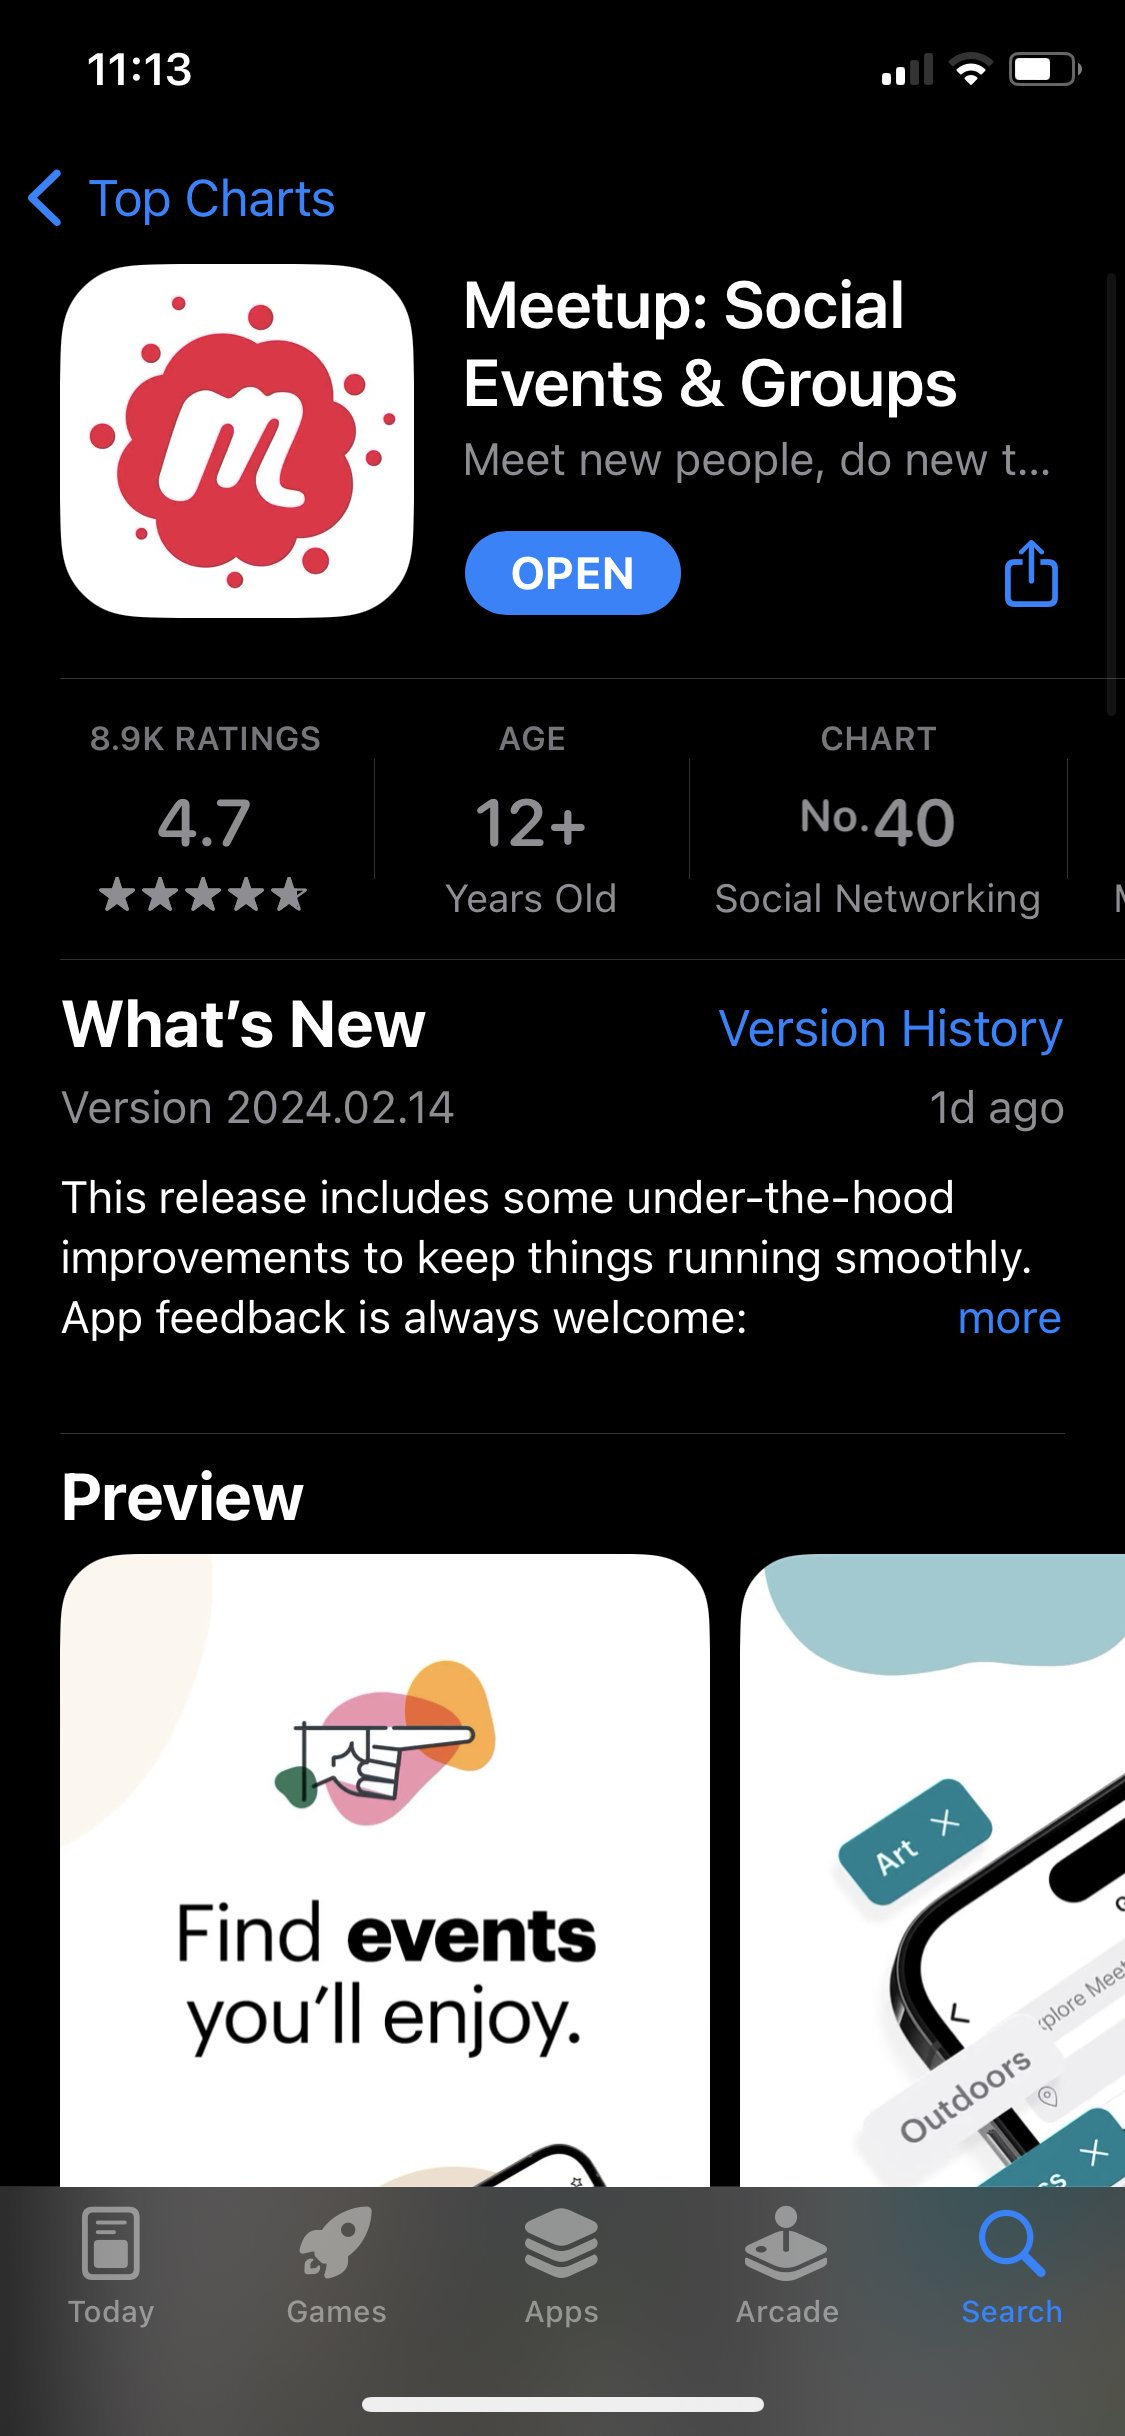
\includegraphics[cframe=black 2pt,width=0.3\linewidth]{images/estadodelarte/meetupappstore.jpeg}
  \caption{Meetup en la App Store}
  \label{fig:meetup_appstore}
\end{figure}
Actualmente, Meetup se cuenta entre las aplicaciones más populares tanto en iOS como en Android, 
ubicándose dentro del top 50 de aplicaciones en la categoría de redes sociales en la App Store de Apple. Meetup ha recaudado \verb|$|15.62 millones a lo largo de 9 rondas de financiación. 
Su última ronda de financiación fue el 11 de enero de 2024. La valoración de Meetup en noviembre de 2017 fue de entre \verb|$|156 y \verb|$|200 millones.\cite{REF11}

Entre las características de Meetup podemos encontrar las siguientes:

\begin{itemize}
  \item \textbf{Organización de grupos:} Los usuarios pueden formar y unirse a grupos basados en intereses comunes.
  \item \textbf{Planificación de eventos:} Los organizadores pueden planificar eventos dentro de su grupo, estableciendo la fecha, la hora, el lugar y los detalles del evento.
  \item \textbf{RSVP para eventos:} Los usuarios pueden confirmar su asistencia a los eventos y ver quién más planea asistir.
  \item \textbf{Comunicación:} Los organizadores y los miembros del grupo pueden comunicarse a través de mensajes dentro de la plataforma, permitiendo la coordinación y el intercambio de información.
  \item \textbf{Categorización de grupos:} Los grupos pueden ser categorizados en base a una variedad de intereses y temas, facilitando a los usuarios encontrar grupos que coincidan con sus intereses.
  \item \textbf{Calendario de eventos:} Los eventos futuros se muestran en un calendario, permitiendo a los usuarios ver los próximos eventos de un vistazo.
  \item \textbf{Eventos locales y virtuales:} Meetup permite la organización de eventos tanto en persona como virtuales, ofreciendo flexibilidad a los usuarios y organizadores.
  \item \textbf{Fotos y comentarios de eventos:} Después de un evento, los asistentes pueden publicar fotos y comentarios, proporcionando un registro de la actividad del grupo y permitiendo a los miembros interactuar después del evento.
\end{itemize}
\begin{figure}[H]
        \centering
        
\includegraphics[width=.5\linewidth]{images/Meetup_Logo.png}
        \caption{Logo de Meetup}
        \label{fig:meetup_logo}
    \end{figure}


\subsection{Strava}

Strava es mucho más que una aplicación para el seguimiento de la actividad física; ha logrado cultivar una comunidad global apasionada de corredores. Sus características sociales juegan un papel crucial en atraer, comprometer y retener a su amplia base de usuarios.

\textbf{Fundación y Enfoque}

Fundada en 2009, Strava originalmente atendía principalmente a ciclistas. Sin embargo, correr rápidamente se convirtió en un enfoque central. La aplicación se posicionó de manera única para aprovechar los conceptos de redes sociales dentro del contexto de corredores en busca de conexión, motivación y competencia amistosa.

\textbf{Cómo Strava Reúne a los Corredores: El Poder de lo Social}

\textit{Experiencia Compartida:} Strava permite a corredores de todos los niveles compartir datos de entrenamiento, rutas y fotos. Esto crea un sentido de experiencia compartida y una plataforma para celebrar logros, incluso entre corredores de todo el mundo.

\textit{Kudos y Comentarios:} Características simples como "kudos" (similares a me gusta) y comentarios generan refuerzo positivo y crean una atmósfera en línea de apoyo. Estas interacciones rápidas aumentan la motivación y construyen conexiones.

\textit{Clubes:} Los clubes de Strava sirven como comunidades de corredores virtuales centradas en ubicaciones específicas, intereses o marcas. Proporcionan un espacio para discusiones en grupo, carreras organizadas y metas compartidas.

\textit{Segmentos y Tablas de Clasificación:} Los segmentos de Strava – porciones designadas de carreras o paseos – convierten cada sendero o camino en una competencia. Las tablas de clasificación fomentan una rivalidad juguetona, empujando a los corredores a esforzarse por mejores personales y una mayor colocación.

\textit{Desafíos:} Los desafíos mensuales y patrocinados por marcas dan a los corredores objetivos para entrenar y construir un sentido de camaradería con otros comprometidos en el mismo desafío.

\textit{Beacon:} La característica de seguridad Beacon permite a los contactos seleccionados rastrear la ubicación de un corredor en tiempo real, fomentando tranquilidad y un sentido indirecto de conexión mientras se entrena solo.

\textbf{Factores Adicionales de Éxito}

\textit{Compatibilidad:} Strava se integra fácilmente con dispositivos GPS populares y relojes inteligentes, aumentando su atractivo y simplificando la entrada de datos.

\textit{Modelo Freemium:} Aunque ofrece características premium, los elementos sociales centrales están disponibles de forma gratuita, facilitando la adopción y el crecimiento de la base de usuarios.

\textit{Énfasis en lo Visual:} Los mapas, gráficos de elevación y fotos hacen que los feeds de actividad sean atractivos, atrayendo a los usuarios de vuelta a la aplicación.

\textbf{Conclusión}

La potente mezcla de elementos sociales de Strava crea un entorno convincente y motivador para los corredores. Entiende la naturaleza social de correr y proporciona formas significativas para que los corredores se conecten, se apoyen mutuamente y celebren logros, todo mientras impulsan el uso de la aplicación.




\subsection{Amigos Social}
Amigos Social es una plataforma social única que enfatiza las conexiones en la vida real y las experiencias compartidas de manera espontánea. A diferencia de las aplicaciones de redes sociales tradicionales, que a menudo se centran en perfiles en línea y contenido curado, Amigos Social busca cerrar la brecha entre las interacciones en línea y los encuentros en persona.

\textbf{Fundación e Historia}

El concepto detrás de Amigos Social surgió en respuesta a un creciente sentido de aislamiento y una falta de compromiso social satisfactorio en nuestro mundo cada vez más digital. Amigos Social comenzó como una plataforma de nicho pero ha visto un crecimiento constante en popularidad, particularmente entre las demografías más jóvenes.

\textbf{Problemas Principales Abordados}

Amigos Social aborda los siguientes problemas centrales dentro del panorama de las redes sociales:

- \textit{Aislamiento y Soledad:} La aplicación crea un camino para la conexión significativa, especialmente para aquellos que luchan por encontrar individuos afines en su entorno inmediato.
- \textit{Torpeza Social:} Minimiza la torpeza de iniciar interacciones sociales al ofrecer una estructura y actividades compartidas para romper el hielo.
- \textit{Aburrimiento y Estancamiento:} La naturaleza espontánea de la aplicación ayuda a los usuarios a salir de las rutinas y descubrir nuevas experiencias.
- \textit{Esfera Social Limitada:} Amigos Social promueve la expansión fácil del círculo social de uno, permitiendo a los usuarios conectarse basados en intereses compartidos y ubicación.

\textbf{Características Destacadas}

Las características sobresalientes de Amigos Social incluyen:

- \textit{Creación y Descubrimiento de Eventos en Tiempo Real:} Los usuarios pueden generar rápidamente eventos sociales con temas variados (deportes, caminatas, encuentros para tomar café, fiestas, etc.) abiertos para que otros se unan en su área.
- \textit{Emparejamiento Basado en Proximidad:} Su interfaz similar a un mapa resalta eventos que ocurren cerca, promoviendo una conexión en el mundo real mientras también permite a los usuarios buscar actividades en otras ubicaciones.
- \textit{Intereses Diversos:} La aplicación apoya una amplia gama de intereses y actividades, asegurando que haya algo para casi todos.
- \textit{Énfasis en la Espontaneidad:} Con eventos siendo creados y unidos en tiempo real, Amigos Social atiende al deseo de conexión social bajo demanda.
- \textit{Seguridad y Consentimiento:} Aunque es más abierta que las plataformas solo por invitación, Amigos Social implementa reportes de usuarios y directrices comunitarias para promover un ambiente seguro y respetuoso.

\textbf{Conclusión}

Amigos Social ofrece una alternativa refrescante para aquellos que buscan interacciones sociales genuinas más allá de las limitaciones de los medios sociales tradicionales. Su énfasis en la espontaneidad, eventos locales y una cultura de experiencias compartidas tiene el potencial de fomentar un sentido de comunidad más fuerte dentro de los entornos del mundo real. La mejora continua de las características de seguridad y la expansión de la base de usuarios probablemente determinarán su éxito a largo plazo.


\section{Conclusión}

Meetup se centra en fomentar las interacciones en el mundo real a 
través de experiencias compartidas. Sin embargo, su enfoque es más 
general y no está diseñado específicamente para la colaboración en 
proyectos concretos o para la formación de grupos con el objetivo de 
realizar actividades específicas a largo plazo. Además, a pesar de su 
popularidad, Meetup no está exento de críticas, particularmente en lo 
que respecta a la experiencia del usuario y a las tarifas de suscripción 
para los organizadores de grupos.

Nuestra propuesta busca abordar estas brechas al proporcionar una 
plataforma más personalizada y simple, orientada a la colaboración en proyectos y 
actividades específicas. A diferencia de Meetup, nuestra aplicación se 
enfocará en la formación de grupos con objetivos a largo plazo y proporcionará 
herramientas robustas para la gestión de proyectos y la comunicación en grupo.